
%<<setup-child, include = FALSE>>=
%library(knitr)
%library(ggplot2)
%set_parent("../style/preamble.Rnw")
%options(digits = 16)
%@


\input{../../2021/style/preamble4tex}
% dependencies: amsmath, amssymb, dsfont
% math spaces
\ifdefined\N
\renewcommand{\N}{\mathds{N}} % N, naturals
\else \newcommand{\N}{\mathds{N}} \fi
\newcommand{\Z}{\mathds{Z}} % Z, integers
\newcommand{\Q}{\mathds{Q}} % Q, rationals
\newcommand{\R}{\mathds{R}} % R, reals
\ifdefined\C
\renewcommand{\C}{\mathds{C}} % C, complex
\else \newcommand{\C}{\mathds{C}} \fi
\newcommand{\continuous}{\mathcal{C}} % C, space of continuous functions
\newcommand{\M}{\mathcal{M}} % machine numbers
\newcommand{\epsm}{\epsilon_m} % maximum error

% counting / finite sets
\newcommand{\setzo}{\{0, 1\}} % set 0, 1
\newcommand{\setmp}{\{-1, +1\}} % set -1, 1
\newcommand{\unitint}{[0, 1]} % unit interval

% basic math stuff
\newcommand{\xt}{\tilde x} % x tilde
\newcommand{\argmin}{\mathop{\mathrm{arg\,min}}} % argmin
\newcommand{\argmax}{\mathop{\mathrm{arg\,max}}} % argmax
\newcommand{\argminlim}{\argmin\limits} % argmin with limits
\newcommand{\argmaxlim}{\argmax\limits} % argmax with limits
\newcommand{\sign}{\operatorname{sign}} % sign, signum
\newcommand{\I}{\mathbb{I}} % I, indicator
\newcommand{\order}{\mathcal{O}} % O, order
\newcommand{\bigO}{\mathcal{O}} % Big-O Landau
\newcommand{\littleo}{{o}} % Little-o Landau
\newcommand{\pd}[2]{\frac{\partial{#1}}{\partial #2}} % partial derivative
\newcommand{\floorlr}[1]{\left\lfloor #1 \right\rfloor} % floor
\newcommand{\ceillr}[1]{\left\lceil #1 \right\rceil} % ceiling
\newcommand{\indep}{\perp \!\!\! \perp} % independence symbol

% sums and products
\newcommand{\sumin}{\sum\limits_{i=1}^n} % summation from i=1 to n
\newcommand{\sumim}{\sum\limits_{i=1}^m} % summation from i=1 to m
\newcommand{\sumjn}{\sum\limits_{j=1}^n} % summation from j=1 to p
\newcommand{\sumjp}{\sum\limits_{j=1}^p} % summation from j=1 to p
\newcommand{\sumik}{\sum\limits_{i=1}^k} % summation from i=1 to k
\newcommand{\sumkg}{\sum\limits_{k=1}^g} % summation from k=1 to g
\newcommand{\sumjg}{\sum\limits_{j=1}^g} % summation from j=1 to g
\newcommand{\summM}{\sum\limits_{m=1}^M} % summation from m=1 to M
\newcommand{\meanin}{\frac{1}{n} \sum\limits_{i=1}^n} % mean from i=1 to n
\newcommand{\meanim}{\frac{1}{m} \sum\limits_{i=1}^m} % mean from i=1 to n
\newcommand{\meankg}{\frac{1}{g} \sum\limits_{k=1}^g} % mean from k=1 to g
\newcommand{\meanmM}{\frac{1}{M} \sum\limits_{m=1}^M} % mean from m=1 to M
\newcommand{\prodin}{\prod\limits_{i=1}^n} % product from i=1 to n
\newcommand{\prodkg}{\prod\limits_{k=1}^g} % product from k=1 to g
\newcommand{\prodjp}{\prod\limits_{j=1}^p} % product from j=1 to p

% linear algebra
\newcommand{\one}{\bm{1}} % 1, unitvector
\newcommand{\zero}{\mathbf{0}} % 0-vector
\newcommand{\id}{\bm{I}} % I, identity
\newcommand{\diag}{\operatorname{diag}} % diag, diagonal
\newcommand{\trace}{\operatorname{tr}} % tr, trace
\newcommand{\spn}{\operatorname{span}} % span
\newcommand{\scp}[2]{\left\langle #1, #2 \right\rangle} % <.,.>, scalarproduct
\newcommand{\mat}[1]{\begin{pmatrix} #1 \end{pmatrix}} % short pmatrix command
\newcommand{\Amat}{\mathbf{A}} % matrix A
\newcommand{\Deltab}{\mathbf{\Delta}} % error term for vectors

% basic probability + stats
\renewcommand{\P}{\mathds{P}} % P, probability
\newcommand{\E}{\mathds{E}} % E, expectation
\newcommand{\var}{\mathsf{Var}} % Var, variance
\newcommand{\cov}{\mathsf{Cov}} % Cov, covariance
\newcommand{\corr}{\mathsf{Corr}} % Corr, correlation
\newcommand{\normal}{\mathcal{N}} % N of the normal distribution
\newcommand{\iid}{\overset{i.i.d}{\sim}} % dist with i.i.d superscript
\newcommand{\distas}[1]{\overset{#1}{\sim}} % ... is distributed as ...


\begin{document}

\lecturechapter{5}{Monte Carlo Integration}
\lecture{CIM1 Statistical Computing}


%\section{Monte Carlo Integration}

\begin{vbframe}{Simple Monte Carlo}

\textbf{Goal:} Calculate $I(f) = \int_a^b f(x)~dx$

\begin{itemize}
\item We define
$$
I(f) = (b - a)\int_a^b f(x)\cdot \frac{1}{b - a}~dx = (b - a)\cdot \E[f(x)]
$$
with $x \sim U(a, b)$
\item With $x_i \overset{iid}{\sim} U(a, b), i = 1, ..., n$ the Monte Carlo estimation is given by

$$
Q_{MC}(f) = \frac{b - a}{n} \sum_{i = 1}^n f(x_i)
$$
\item By \enquote{sampling} $n$ independent random numbers from $U(a,b)$ an estimate for the integral can be calculated.
\end{itemize}

\framebreak

Monte Carlo is a \textbf{non-deterministic} approach. The estimation for the integral $\int_a^b f(x) ~dx$ is subject to randomness:

\begin{itemize}
\item The strong law of large numbers states that $Q_{MC}(f)$ converges almost certainly towards $I(f) = \E[f(x)]$ for $n\to\infty$
\item We can derive the variance from $Q_{MC}(f)$:
\vspace*{-0.2cm}
\begin{eqnarray*}
\text{Var}\left(Q_{MC}(f)\right) &=& \text{Var}\left(\frac{b - a}{n} \sum_{i = 1}^n f(x_i)\right) \\
&\overset{iid}{=}& \frac{(b - a)^2}{n^2}\cdot n \cdot \text{Var}(f(x)) = \frac{(b - a)^2}{n} \sigma^2
\end{eqnarray*}
where $\sigma^2 = \text{Var}(f(x))$ denotes the variance of the random variable $f(x)$ with $x \sim U(a, b)$ which can be empirically estimated by \begin{footnotesize}$\hat \sigma^2 = \frac{1}{n - 1} \sum_{i = 1}^n \left(f(x_i) - \frac{1}{n}\sum_{i = 1}^n f(x_i)\right)^2, x_i \overset{iid}{\sim} U(a, b)$\end{footnotesize}.

\framebreak

% \item Mit $\hat \sigma^2 = \sum_{i = 1}^n \frac{\left(f(x_i) - \frac{1}{n}\sum_{i = 1}^n f(x_i)\right)^2}{n - 1}$ kann Varianz von $Q_{MC}(f)$ geschätzt werden
% \begin{eqnarray*}
% \widehat{\text{Var}}\left(Q_{MC}(f)\right) &=& \frac{(b - a)^2}{n} \cdot \sum_{i = 1}^n \frac{\left(f(x_i) - \frac{1}{n}\sum_{i = 1}^n f(x_i)\right)^2}{n - 1}.
% \end{eqnarray*}

\item If $\sigma^2 < \infty$ the variance of the estimate (and thus also the worst case error of the procedure) approaches $0$ for $n \to \infty$
\item Monte Carlo also works well in multidimensional settings:
\vspace*{-0.2cm}
\begin{itemize}
\item The Monte Carlo integration can simply be generalized to multidimensional integrals $\int_\Omega f(\bm{x}) ~ d\bm{x}$ with $\Omega \subset \R^d$ by drawing the random variables uniformly distributed in the $d$-dimensional space $\Omega$.
\item The variance is then
$$
    \text{Var}\left(Q_{MC}(f)\right) = \frac{V^2}{n} \sigma^2, \quad V = \int_\Omega ~ d\bm{x}
$$
\item In particular, the speed of convergence for the variance \textbf{does not} depend on the dimension of the function to be integrated.
\end{itemize}
\end{itemize}
\end{vbframe}



\begin{vbframe}{Hit-or-Miss}

\textbf{Idea:}

We draw $n$ independently uniformly distributed data points from a rectangle enclosing our function:

\begin{center}
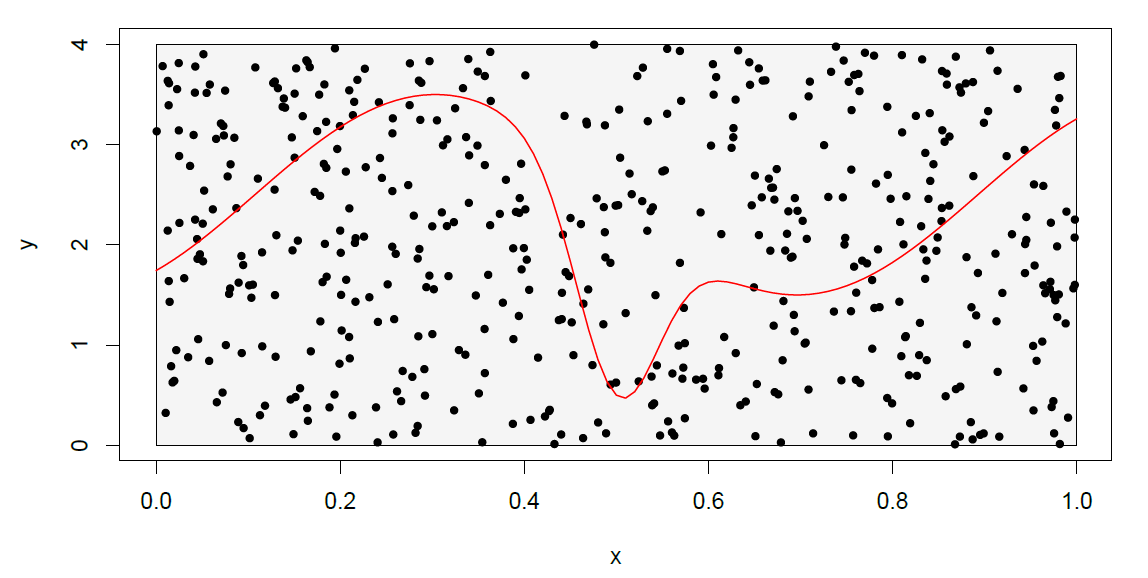
\includegraphics[width =0.7\textwidth]{figure_man/hitormiss.png}
\end{center}

\framebreak

\textbf{\enquote{Hit-or-Miss} Approach:}



We still consider the integral $\int_a^b f(x) dx$. We assume that $0 \le f(x) \le c$. If we count the number of hits (the points underneath the curve), we obtain the integral by:

$$
  I(f) \approx \frac{Hits}{n} \cdot \text{area of the rectangle} = \frac{\sum_i \mathbf{1}_{y_i \le f(x_i)}}{n} \cdot c \cdot (b - a)
$$

\vspace*{-0.3cm}

\begin{center}
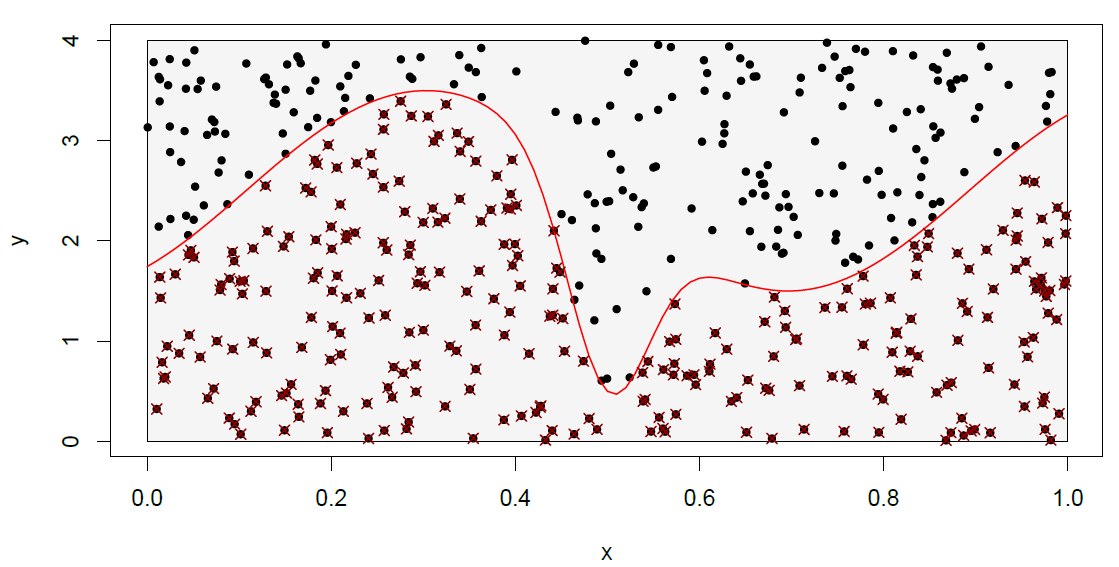
\includegraphics[width =0.7\textwidth]{figure_man/hitormiss2.png}
\end{center}


\framebreak


\footnotesize
\begin{verbbox}
m$estimate # Estimation of area
## [1] 2.288
m$hits # Number of points underneath the curve
## [1] 286
\end{verbbox}
\col


\normalsize
$$
  I(f) \approx \frac{286}{500} \cdot \text{1 * 4} = 2.288
$$

This naive method works well for simple examples, but error rates are high for more complex applications.

\framebreak






% \framebreak
%
% \textbf{Anwendung:} Bayesian Computations
%
% \lz
%
% \textbf{Ziel:} Berechnung des Posterior-Erwartungswert $
% E(\theta | \xv) = \int \theta f(\theta | \xv)d\theta$
%
% \lz
%
% \begin{itemize}
% \item Angenommen, unabhängige Samples $\theta^{(1)}, \ldots, \theta^{(T)}$ aus
% $f(\theta | \xv)$ können einfach erzeugt werden.
% \item Eine Monte-Carlo-Schätzung des Posterior-Mittelwerts ist dann
% $$
% \hat{E}(\theta | \xv) = \frac{1}{T} \sum_{t = 1}^T \theta^{(t)}.
% $$
% \item Der Schätzer konvergiert zum wahren Posterior-Mittelwert konvergiert für $T \rightarrow \infty$ (Gesetz der großen Zahlen).
% \end{itemize}
% % Fehlerrate ist $\mathcal{O}(\frac{1}{\sqrt{T}})$. Relativ langsamer Algorithmus, aber sehr einfach,
% % falls Zufallszahlengenerator e\xvistiert.
% %
% \framebreak
%
%
% Die allgemeinere Form
%
% $$
% \hat{E}(g(\theta) | \xv) = \frac{1}{T} \sum_{t = 1}^T g(\theta^{(t)})
% $$
%
% ist ebenfalls konsistent.
%
% \lz
%
% Somit kann beispielsweise die Posterior-Varianz
% $$
% \widehat{Var}(\theta | \xv) = \hat{E}(\theta^2 | \xv) - \hat{E}(\theta | \xv)^2.
% $$
%
% \lz
%
% oder die kumulative Posterior-Verteilungsfunktion
%
% $$
% P(\theta \leq \theta_0) | \xv)
% $$
% mit Hilfe von Indikatorfunktionen $g(\theta) = I_{(-\infty, \theta_0]}(\theta)$ berechnet werden.
%
% \frembreak
%
%
% Wenn die Samples $\theta^{(t)}$ nicht wirklich unabhängig sind, betrifft das lediglich
% die Genauigkeit von $\hat{E}(g(\theta) | \xv)$.

\framebreak

\textbf{Advantages:}
\begin{itemize}
\item Monte Carlo integration does not require continuity for $f$
\item Error does not depend on the dimension (in contrast to deterministic quadrature formulas), but only on the variance of the function $f$ and the number of simulations $n$
\begin{itemize}
\item $\to$ Improve precision through high number of simulations
\item $\to$ Improve precision by reducing variance
\end{itemize}
\end{itemize}

\textbf{Disadvantages:}
\begin{itemize}
\item Relatively slow convergence rates
% \item setzt voraus, dass von $f(\theta|\xv)$ simuliert werden kann
\end{itemize}


% Trapezregel und Rechtecksregel haben Fehler der Ordnung $h^2$ (auch in höheren Dimensionen).
%
% \lz
%
% Das entspricht:
% \begin{itemize}
% \item Eindimensional:  $\mathcal{O}(\frac{1}{N^2})$.
% \item Zweidimensional: $\mathcal{O}(\frac{1}{N})$.
% \item Vierdimensional: $\mathcal{O}(\frac{1}{\sqrt N})$.
% \end{itemize}
% Dies ist der \textbf{Fluch der Dimensionalität}.

% \lz
%
% Vorteile der Monte-Carlo-Integration:
% \begin{itemize}
% \item Konvergenzrate unabhängig von Dimension. Ab Dimensionen 4 wird Monte-Carlo kompetitiv.
% \item Numerische Quadratur am besten, wenn $f$ glatt, z.B. Simpson $\mathcal{O}(h^4)$.
% \end{itemize}

\begin{center}
<<echo=F, include = FALSE>>=
set.seed(333)
@
<<include = FALSE>>=
T = 10000; shape = 2; rate = 1 / 2
theta = rgamma(T, shape = shape, rate = rate)
@
<<out.width = '80%', fig.align = "center", echo=F, include = FALSE>>=
hist(theta, freq = FALSE, ylim = c(0, 0.2), main = "")
lines(density(theta))
@
\end{center}

% \framebreak
%
% Schätzung des Posterior-Erwartungswertes $\hat{E}(\theta | \xv)$

<<include = FALSE>>=
(Etheta = mean(theta)) # MC estimator
(se.Etheta = sqrt(var(theta) / T)) # Variance of MC estimator
shape * 1 / rate # Theoretical expectation

@


% \framebreak
%
% Schätzung des Posterior-Verteilungsfunktion $P(\theta > 5) | \xv)$

<<include = FALSE>>=
(Ptheta = mean(theta > 5)) # MC Estimator
(se.Ptheta = sqrt(var(theta > 5) / T)) # Variance of MC estimator
1 - pgamma(5, shape = shape, rate = rate) # theoretical value
f = function(x) { dgamma(x, shape = shape, rate = rate) }
integrate(f, 5, Inf) # Numerical integration in R
@

% \framebreak

% \textbf{Highest Posterior Density (HPD)}

% \lz

% HPD Intervalle können ebenfalls konsistent geschätzt werden. HPD Intervalle haben die minimale
% Range von allen möglichen Konfidenzintervallen für ein vorgegebenes $\alpha$, z.B.,
% $\alpha = 0.95$.
% \begin{itemize}
% \item Sortiere $\theta^{(1)} \leq \cdots \leq \theta^{(T)}$.
% \item Empirische Konfidenzintervalle mit $\alpha = 0.95$ und $T = 100$:
%   {\small
%   $$
%   [\theta^{(1)}, \theta^{(95)}], [\theta^{(2)}, \theta^{(96)}], [\theta^{(3)}, \theta^{(97)}],
%     [\theta^{(4)}, \theta^{(98)}], [\theta^{(5)}, \theta^{(99)}], [\theta^{(6)}, \theta^{(100)}].
%   $$
%   }
% \item HPD ist jenes Intervall mit der geringsten Breite.
% \end{itemize}

% \lz

% Der Posterior Modus kann ebenfalls mit Hilfe des HPD-Intervalls und bspw.\ $\alpha = 0.99$
% geschätzt werden. Der Modus ist dann in der Mitte des Intervalls (nicht unbedingt elegant, aber
% auch nicht viel schlechter wie andere Methoden).

% \framebreak

% <<>>=
% hpd = function(x, prob = 0.05) {
%   T = length(x)
%   x = sort(x)
%   gap = max(1, min(T - 1, round(T * (1 - prob))))
%   j = 1:(T - gap)
%   i = which.min(x[j + gap] - x[j])
%   int_hpd = x[c(j[i], j[i] + gap)]
%   int_et = quantile(x, prob = c(prob / 2, 1 - prob / 2))
%   names(int_hpd) = names(int_et) = c(
%     paste(round(prob / 2 * 100, 2), "%", sep = ""),
%     paste(round((1 - prob / 2) * 100, 2), "%", sep = "")
%   )
%   int = rbind("HPD" = int_hpd, "Equi-tailed" = int_et)
%   return(int)
% }
% @

% \framebreak

% <<>>=
% hpd(theta)
% @
% \begin{center}
% <<echo=FALSE>>=
% hist(theta, freq = FALSE, ylim = c(0, 0.2), main = "")
% lines(density(theta))
% int = hpd(theta)
% library("colorspace")
% col = rainbow_hcl(2)
% abline(v = int[1, ], col = col[1], lwd = 2)
% abline(v = int[2, ], col = col[2], lwd = 2)
% legend("topright", c("HPD", "Equi-tailed"), lwd = 2, col = col,
%   box.col = NA, bg = NA)
% @
% \end{center}

% \framebreak

% <<>>=
% int = hpd(theta, prob = 0.99)
% (mode = mean(int["HPD", ])); (shape - 1) * 1 / rate
% @
% \begin{center}
% <<echo=FALSE>>=
% hist(theta, freq = FALSE, ylim = c(0, 0.2), main = "")
% lines(density(theta))
% abline(v = mode, col = col[1], lwd = 2)
% legend("topright", c("mode"), lwd = 2, col = col[1],
%   box.col = NA, bg = NA)
% @
% \end{center}

% \framebreak

% \textbf{Importance Sampling}
%
% Erweiterung von Monte-Carlo, wenn Samples nicht direkt von $f(\theta | \xv)$ erzeugt werden können.
%
% \lz
%
% Wenn Zufallszahlen aus $f^\star(\theta)$ generiert werden können, dann kann der Posterior-Erwartungswert durch
% $$
% E(g(\theta) | \xv) = \int g(\theta) \frac{f(\theta | \xv)}{f^\star(\theta)} f^\star(\theta)d\theta
% $$
% berechnet werden. Die Schätzung basierend auf den Samples aus $f^\star(\theta)$ ist dann
% $$
% \hat{E}(g(\theta) | \xv) = \frac{1}{\sum_{t = 1}^T \omega_t} \sum_{t = 1}^T \omega_t g(\theta^{(t)}),
% $$
% mit $\omega_t = f(\theta^{(t)} | \xv) / f^\star(\theta^{(t)})$.
%
% \framebreak
%
% <<>>=
% T = 10000; shape = 2; rate = 1 / 2
% u = runif(T, 0, 1000)
% w = dgamma(u, shape = shape, rate = rate) / (1 / 1000)
% (Etheta = sum(u * w) / sum(w))
% shape * 1 / rate
% @
%
% \framebreak

% \textbf{Slice Sampling}

% Slice Sampling beruht auf der Eigenschaft, dass Zufallszahlen aus einer Dichtefunktion auch mittels
% gleichverteilter Zufallszahlen die unterhalb von $f(\theta | x)$ liegen erzeugt werden können.

% \lz

% D.h., alle Punkte $(\theta, u)$ für die gilt $0 \leq u \leq f(\theta | x)$.

% \lz

% Algorithmus (stark vereinfacht):
% \begin{itemize}
% \item Initialisiere Startwert $\theta^{(0)}$.
% \item Sample $u \sim U(0, f(\theta^{(t)} | x))$.
% \item Sample $\theta^{(t + 1)} \sim U(s)$ mit $s = \{ \theta^\star : f(\theta^\star | x) \leq u \}$.
% \end{itemize}

% \framebreak

% <<fig.height=3.5, fig.width=5.95>>=
% f = function(x) {
%   dgamma(x, shape = 2, rate = 1 / 2)
% }
% curve(f, 0, 20)
% @
% <<>>=
% find.slice = function(x, fx, f, w = 0.001) {
%   left = right = x
%   repeat {
%     if(f(left) <= fx) break
%     left = left - w
%   }
%   repeat {
%     if(f(right) <= fx) break
%     right = right + w
%   }
%   c(left, right)
% }
% @

% \framebreak

% \begin{center}
% <<>>=
% find.slice(5, 0.08, f)
% @
% <<echo=FALSE, fig.height=3.5, fig.width=5.95>>=
% curve(f, 0, 20)
% slice = find.slice(5, 0.08, f)
% lines(slice, f(slice))
% points(slice, f(slice), pch = 16)
% @
% \end{center}

% \framebreak

% <<>>=
% slicer = function(n, f, w = 0.001, start = 1) {
%   x = start
%   samples = NULL
%   for(i in 1:n) {
%     u = runif(1, 0, f(x))
%     slice = find.slice(x, u, f, w)
%     x = runif(1, slice[1], slice[2])
%     samples = c(samples, x)
%   }
%   return(samples)
% }
% @

% \framebreak

% <<fig.height=3.5, fig.width=5.95>>=
% x = slicer(1000, f, start = 2)
% @
% \begin{center}
% <<echo=FALSE, fig.height=3.5, fig.width=5.95>>=
% hist(x, freq = FALSE, main = "", ylim = c(0, 0.2))
% lines(density(x))
% curve(f, 0, 20, col = "red", add = TRUE)
% @
% \end{center}
\end{vbframe}


\endlecture
\end{document}
